\documentclass[conference]{IEEEtran}
\IEEEoverridecommandlockouts

\usepackage{amsmath,amssymb,amsfonts}
\usepackage{algorithmic}
\usepackage{graphicx}
\usepackage{textcomp}
\usepackage{xcolor}

\usepackage[english]{babel}
\usepackage{csquotes}
\usepackage[
    backend=biber, 
    natbib=true,
    style=numeric,
    sorting=none,
]{biblatex}
\addbibresource{Bibliography.bib}


\ifCLASSOPTIONcompsoc                         \usepackage[caption=false,font=normalsize,labelfont=sf,textfont=sf]{subfig}
\else
\usepackage[caption=false,font=footnotesize]{subfig}
\fi


\def\BibTeX{{\rm B\kern-.05em{\sc i\kern-.025em b}\kern-.08em
    T\kern-.1667em\lower.7ex\hbox{E}\kern-.125em}}
    

\begin{document}

\title{
    Comparative Study of Machine Learning Techniques For Water Potability Prediction

    % A Comparative Study of Binary Classification Algorithms for Water Potability Prediction
}

\author{
    \IEEEauthorblockN{  
    Ying Ying Lai
    }
    \IEEEauthorblockA{
        \textit{
            School of Information Technology
        }\\
        \textit{
            Monash University Malaysia
        }\\
        ylai0018@student.monash.edu
    }   
}
\maketitle

% #########################################
% --------------- ABSTRACT ---------------
% #########################################
\begin{abstract}
In recent years, Internet Of Things (IoT) has become increasingly popular due to its smart application in various fields. Modern water treatment plant has been using smart sensors for real-time water quality monitoring and prediction to ensure the water is appropriate for its intended purpose. In this paper, the performance of various machine learning (ML) algorithms on the task of predicting water potability are compared and discussed. The techniques chosen including but not limited to Logistic Regression, Random Forest, K-Nearest Neighbours (KNN), Support Vector Machine (SVM) and Artificial Neural Network(ANN). The accuracy of these models are determined using evaluation metrics such as the accuracy, precision, recall and f1 score. The results shown that the SVM model performed the best with the highest accuracy and lesser training time as compared to the more complex classification algorithms. It is able to achieve the accuracy of 98.16\%, followed by Random Forest with an accuracy of 97.53\%.
\end{abstract}


\begin{IEEEkeywords}
water quality prediction, binary classification, SVM, Random Forest, logistic regression, neural network, IoT
\end{IEEEkeywords}

% #########################################
% ------------- INTRODUCTION -------------
% #########################################
\section{Introduction}
Water is an essential resource that is needed to sustain life on earth. In recent years, Malaysia is experiencing an increased demand for water as its supply has changed from one of relative abundance to one of scarcity~\cite{ahmed_siwar_2014}. In fact, this is a global issue that is already affecting every continent. Water is needed for agriculture, energy production, recreation, and manufacturing~\cite{anang2019factors} and a lack of access to clean water can threatens human well-being, economic productivity as well as the ecological communities. To make matters worse, abrupt climate change coupled with massive population growth and rapid urban development further aggravate the issue, pushing governments to actively look for innovative and collaborative solutions to tackle this issue.

In an effort to achieve sustainable water use and management, governments and environmental organizations have been exploring the potential reuse of wastewater post-treatment for different end use. An important aspect in determining the suitability of water usage is the monitoring and prediction of water quality by analysing its chemical, physical and biological properties. The integration of IoT allows these information to be collected over an extended period of time and often the data exist in the form of multivariate time-series datasets~\cite{zhou2018water}. Artificial Intelligence (AI) offers significant opportunities to help improve the classification and prediction of water quality by developing a dependable approach for forecasting water quality as accurately as possible~\cite{nasir2022water}. 

This study focuses on predicting the potability of water based on 20 water parameters, which includes but not limited to the aluminium, ammonia, copper and selenium content of the water, using various machine learning techniques. The models are fine-tuned to achieve its optimal performance before evaluating their accuracy. 

Section II of this paper provides some background of the project topic and literature review of related works. Section III dives into the research methodology, where I will be explaining on the data collection methods, pre-processing steps, and classification methods. Then, the performance of the models will be discussed in section IV, along with their respective test scores and visual representations of the evaluation metrics. Lastly, Section V concludes the paper with a brief summary of this research findings.
     
% #########################################
% --------------- BACKGROUND -------==-----
% #########################################
\section{Background}    
% -------------- Water Quality Monitoring -------------
\subsection{Water Quality Monitoring}
Depending on the designated usage, water specifications for different applications possess a set of standards that must be met in order to be considered safe. These guidelines are based on scientific research and epidemiological findings, and as such provide guidance for making risk management decisions related to the protection of public health and the preservation of the environment~\cite{lee1982water}. For example, water bodies such as rivers, lakes, and streams have specific quality standards that indicate their quality to ensure that the amount of pollutants presence is within the tolerance limit of water species~\cite{aldhyani2020water}. On the other hand, water must not be too saline nor contain toxic materials to 
be qualified for irrigation purposes to protect the plant and ecosystems~\cite{aldhyani2020water}. Hence, continuous monitoring, evaluation and prediction of water quality are necessary. 

% -------- Traditional Water Sampling and Testing ---------
\subsection{Traditional Water Sampling and Testing}
Traditional wastewater quality monitoring methods involve manual collection of water samples at different locations, followed by laboratory analytical techniques in order to characterize the water quality~\cite{martinezetal}.
Besides being labour intensive, laboratory analysis is time consuming and high costs is needed for labour, maintenance and operations of equipment. Considering all water quality parameters is also unrealistic because it is not only expensive and technically difficult but also fails to deal with the variability in water quality~\cite{zhu2022review}. Besides that, this method does not offer real-time water quality detection, hence responsible authorities will not be able to take immediate action if the water is unsafe for usage.

% ------ IoT based Water Quality Monitoring System -------
\subsection{IoT based Water Quality Monitoring System}
With the advancement in technology, a real-time, cost-effective water quality monitoring system can be easily deployed. This is achieved by embedding sensors that sent its sensor readings to the server for monitoring and analytical purposes. In recent years, the vision of the Internet of Things (IoT) augmented with advances in software technologies, such as service-oriented architecture (SOA), software as a service (SaaS), cloud computing, and others, has stimulated the development of smart water quality monitoring systems~\cite{martinezetal}. 

% ------ Machine Learning in Water Quality Prediction -------
\subsection{Machine Learning in Water Quality Prediction}
Based on Zhu et al.~\cite{zhu2022review}, the integration of sensors in water treatment plant has multiple benefits such as continuous water quality monitoring and prediction, pollutant source tracking, and pollutant concentration estimation, water resource allocation and water treatment technology optimization. These sensors generate a high volume of multivariate data. Manual water quality analysis are no longer preferred due to human's inability to handle such complex data. Besides being more error-prone, this process is both cost- and time-consuming.

These limitations are overcome by machine-learning based models, which is widely known to increase productivity and efficiency in many fields. It's ability to correctly interpret external data, to learn from such data, and to use those information to achieve specific goals and task through flexible adaptation~\cite{haenlein2019brief} allows the model to achieve better performance and accuracy in evaluation and analysis~\cite{geetha2020overview}. 

Machine learning can be divided into two main classes, which is supervised and unsupervised learning ~\cite{berry2019supervised}. In the case of water quality prediction, we will be looking into supervised learning algorithms since all data in the dataset are labeled. The aim is to study the relationships or correlation between the paired labels and generate a predictive model. The model is then used to predict the result based on a set of input data. Data classification and regression apply the concept of supervised learning to generate a model, while utilising algorithms such as naive Bayes, logistic regression, decision tree, random forest, support vector machine, k-nearest neighbour and support vector machine ~\cite{zhu2022review}. 

Unlike manual water sampling, ML models are able to consistently provide more accurate evaluation results despite the complexity of the dataset. The feasibility and effectiveness of these models demonstrates its potential to be used as a tool in water quality evaluation~\cite{zhu2022review} since the evaluation process often involves large multivariate time-series dataset. Multiple parameters will need to be considered when determining water quality because a slight change in the water parameters level can potentially affect the suitability of the water for a certain usage. Lastly, the use of ML models over manual water sampling and analysis also has the benefits of reducing labour cost, less error-prone and more time-efficient.

% -------------------- Related Works ---------------------
\subsection{Related Works}
In recent years, many research has been carried out to study how different types of machine learning (ML) classification algorithms can affect the accuracy of the model in water quality prediction. Zai C. et. al~\cite{zai2022prediction} found that Decision Tree Algorithm performed decently well in evaluating the water quality index. It has a R-squared error $ R^{2}$ score of 72\% and Root Mean Square Error (RMSE) score of 0.41, which denotes excellent performances in the proposed models for forecasting IWQ showing to other models that have been proposed in the literature. 

Nasir N. et. al~\cite{nasir2022water} investigated the performance of various machine learning algorithms on predicting the water quality index (WQI) using seven different water parameters. The classifiers that are implemented include Support Vector Machine (SVM), Random Forest (RF), Logistic Regression (LR), Decision Tree (DT), CATBoost, XGBoost, and Multilayer Perceptron (MLP).Results show that the CATBoost model has the highest accuracy of 94.51\%. The accuracy of all classifier reached 100\% when implemented along with stacking ensemble models.
    
A similar study is carried out by Poudel D.~\cite{poudelcomparison} to study water potability using a dataset with different water parameters. The research compares the efficiency of Logistic Regression (LR), K-Nearest Neighbours (KNN) and Random Forest (RF) and Artificial Neural Network (ANN) in predicting dataset that are statistically imputed. 

Zhou J. et. al~\cite{zhou2018water} proposed a model that uses IGRA for feature selection and LSTM for water quality prediction. IGRA calculates the similarity and proximity by relative area change ratio, whereas LSTM is faster at converging to the optimal solution, especially when dealing with time sequence prediction problems. This model takes full advantage of the multivariate correlation and time sequence of water quality information, and is ideal for multi-class classification problem. 

Another research by Aldhyani et. al~\cite{aldhyani2020water} studied the performance of various machine learning algorithms on different water types such as surface water, wastewater and drinking water. The performances are evaluated based on the recognition rate, training time and robustness, and it is revealed that ANN has the highest recognition rate and and SVM is very robust to noise. These methods are widely applied in large dimension to dynamically monitor the quality and safety of drinking water in real-time since they have the best training performances for predicting the potability of water among the other algorithms~\cite{bouamar2007evaluation}. 

% #########################################
% -------------- METHODOLOGY ------==-----
% #########################################
\section{Methodology}
The aim of this paper is to study the accuracy of 9 different binary classification algorithms in predicting the potability of water based on 20 water chemical properties. The models were implemented using Logistic Regression (LR), Naive Bayes (NB), Decision Tree (DT), Random Forest (RF), K-Nearest Neighbours (KNN), Support Vector Machines (SVM), Extreme Gradient Boosting (XGBoost), and the Multi-layer Perceptron (MLP) algorithms. The following sections include discussions on the data pre-processing steps, classification techniques and evaluation metrics used to compare the performance of the models.
 
% ---------------- Dataset Selection -----------------
\subsection{Dataset Selection}
The dataset chosen provides information on the safety of water for drinking purposes. It is a public dataset that can be downloaded from Kaggle website~\cite{kaggledataset}. It contains a total of 7998 rows of water sample and the potability of each sample is determined by 20 continuous features. The classification feature is potability with values of either 0 or 1, where 0 denotes non-potable, and 1 denotes potable. The features and their respective datatype are shown in Table~\ref{table:water_parameters}. 

\begin{table}[htbp]
    \renewcommand{\arraystretch}{1.3}
    \caption{Water Parameters In Dataset (Raw)}
    \label{table:water_parameters}
    \centering
    \renewcommand{\arraystretch}{1.3}
    \setlength{\tabcolsep}{10pt}
    \begin{tabular}{c|c}
        \hline 
        \bfseries Parameter & \bfseries Datatype \\
        \hline  \hline
        aluminium & float64\\
        ammonia & object\\
        arsenic & float64\\
        barium  & float64\\
        cadmium & float64\\
        chloramine & float64\\
        chromium & float64\\
        copper & float64\\
        fluoride & float64\\
        bacteria & float64\\
    \hline
    \end{tabular}
    \quad
    \setlength{\tabcolsep}{10pt}
    \begin{tabular}{c|c}
        \hline
        \bfseries Parameter & \bfseries Datatype \\
        \hline \hline
        viruses & float64\\
        lead & float64\\
        nitrates & float64\\
        nitrites & float64\\
        mercury & float64\\
        perchlorate & float64\\
        radium & float64\\
        selenium & float64\\
        silver & float64\\
        uranium & float64\\
        \hline
    \end{tabular}
\end{table}

% ---------------- Data Pre-proccessing -----------------
\subsection{Data Pre-processing}
Real-world data often contains missing values, outliers and misleading data, and sometimes there is no guarantee to the reliability and credibility of the data sources. These issues may drastically affect the performance and accuracy of the machine learning model since the training outcome depends heavily on the dataset ~\cite{gawhade2022}. Data pre-processing removes irrelevant entries by cleaning (i.e., removing outliers) and labeling the data \cite{nasir2022water}.
Below are the steps taken during pre-processing:

% ###### Handling Categorical Variable
\subsubsection{Categorical Variable}
The column for the water parameter, \emph{ammonia}, and potability, \emph{is\_safe}, have a datatype of object. Since the dataset contains information regarding the potability of water samples and their corresponding features values, the column for potability should be stored as either 0 or 1, and the \emph{ammonia} column is a continuous variable that stores a range of numeric. Therefore, both the column were casted as \emph{float64}.  

% ###### Handling Missing Values
\subsubsection{Missing Values}
In this dataset, only 3 out of 7998 water samples contain \emph{Null} values, which is less than 0.01\% of the entire dataset. Therefore, I decided to remove the instances of water samples instead since removing them will not cause a significant change in the training result.
  \begin{table*}[htbp]
    % \renewcommand{\arraystretch}{1.3}
    \caption{Sample Dataset}
    \label{table:dataset}
    \centering
    \begin{tabular}{c c c c c c c c c c c }
        \hline 
        \bfseries aluminium & \bfseries ammonia & \bfseries arsenic & \bfseries barium & \bfseries cadmium & \bfseries chloramine & \bfseries chromium & \bfseries copper & \bfseries flouride & \bfseries bacteria & \bfseries viruses \\
        \hline  \hline
          1.65 & 9.08 & 0.04 & 2.85 & 0.01 & 0.35 & 0.83 & 0.17 & 0.05 & 0.2 & 0.0\\
          2.32 & 21.16 & 0.01 & 3.31 & 0.0 & 5.28 & 0.68 & 0.66 & 0.9 & 0.65 & 0.65\\ 
          1.01 & 14.02 & 0.04 & 0.58 & 0.01 & 4.24 & 0.53 & 0.02 & 0.99 & 0.05 & 0.0\\ 
          1.36 & 11.33 & 0.04 & 2.96 & 0.0 & 7.23 & 0.03 & 1.66 & 1.08 & 0.71 & 0.71\\ 
          0.92 & 24.33 & 0.03 & 0.2 & 0.01 & 2.67 & 0.69 & 0.57 & 0.61 & 0.13 & 0.0\\ 
    \hline
    \end{tabular}
    \quad
    \begin{tabular}{c c c c c c c c c c }
        \hline
         \bfseries lead & \bfseries nitrates & \bfseries nitrites & \bfseries mercury & \bfseries perchlorate & \bfseries radium & \bfseries selenium & \bfseries silver & \bfseries uranium & \bfseries is\_safe \\
        \hline \hline 
        0.05 & 16.08 & 1.13 & 0.01 & 37.75 & 6.78 & 0.08 & 0.34 & 0.02 & 1.0\\
        0.1 & 2.01 & 1.93 & 0.0 & 32.26 & 3.21 & 0.08 & 0.27 & 0.05 & 1.0\\
        0.08 & 14.16 & 1.11 & 0.01 & 50.28 & 7.07 & 0.07 & 0.44 & 0.01 & 0.0\\
        0.02 & 1.41 & 1.29 & 0.0 & 9.12 & 1.72 & 0.02 & 0.45 & 0.05 & 1.0\\
        0.12 & 6.74 & 1.11 & 0.0 & 16.9 & 2.41 & 0.02 & 0.06 & 0.02 & 1.0\\
        \hline
    \end{tabular}
\end{table*}

% ###### Data Augmentation
\subsubsection{Imbalanced dataset}
Figures~\ref{fig_before} shows that the dataset has a highly imbalanced data distribution, where the number of water samples for potable water is significantly lower than that of the non-potable water. To overcome this, oversampling technique is applied to the minority class to generate new samples, aiming to achieve a well-balanced class distribution~\cite{douzas2018improving}. The synthetic minority oversampling technique (SMOTE) algorithm is chosen to perform oversampling due to its ability to prevent over-fitting by creating samples from the interpolation between the existing samples and their neighbors~\cite{nasir2022water}.
\begin{figure}[htbp]
    \centering
    \subfloat[Before oversampling]{
        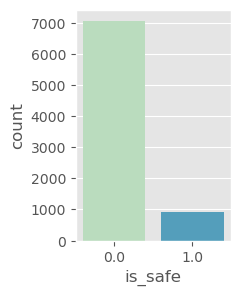
\includegraphics[width=1.2in]{graphs/ori_data_ratio.png}
        \label{fig_before}
    }
    % \hfil
    \subfloat[After oversampling]{
        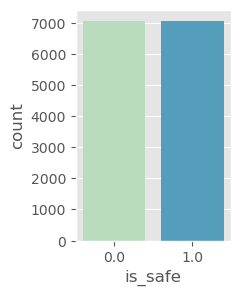
\includegraphics[width=1.2in]{graphs/resampled_ratio.png}
        \label{fig_after}
    }
    \caption{Potability Class Distribution} \label{fig_data_num}
\end{figure}

% ###### Splitting Dataset
\subsubsection{Data-Split}
The dataset is divided into training and testing sets with a proportion of 70\% and 30\% respectively, resulting in 9917 training data and 4251 testing data.

% ##### Data Normalisation
\subsubsection{Normalisation}
Data Normalisation is done by scaling and translating each feature in the training set individually to a range between the minimum and maximum values ~\cite{scikit}. The transformation is given by:
\begin{align*}
X\_std = &(X - X.min(axis=0)) / \\
&(X.max(axis=0) - X.min(axis=0)) \\
X\_scaled = &X\_std * (max - min) + min
\end{align*}

% ------------------------ CLASSIFICATION ------------------------
\subsection{Classification}
A brief description of each classification technique is presented in the section below.

\subsubsection{Naive Bayes}
A probabilistic classification technique used to determine is a data point falls into a particular class. It is based on the Bayes Theorem, which is used to calculate conditional probability. Many Naive Bayes are available, however, the Gaussian Naive Bayes is used in this study and the likelihood of each feature is assumed to be: 
\[
P(x_i|y) = \frac{1}{\sqrt(2\pi\sigma^2_y \exp(-\frac{(x_i-\mu_y)^2}{2\sigma^2_y})} 
\]

\subsubsection{Logistic Regression}
A standard classification classifier that uses the probabilistic statistics of the data to predict binomial outcomes. The standard logistic function is an S- shaped curve, which is given by the equation:
\[
\frac{1}{1 + e^{-x}} = \frac{e^x}{1+e^x}
\]

\subsubsection{Decision Tree}
Decision Tree is used for both classification and regression. It first learn to generate a decision tree from a set of training samples that have been classified, and the tree obtained is for used as a model to classify other unclassified data~\cite{lan2020comparative}. A decision tree starts with internal nodes representing a test of each features, moving down branches which represents the output, and the leaves nodes contain the resulting decisions. Due to the presence of variance, the downside to this method is that they tend to cause overfitting. Besides that, decision tree can become costly especially when the data set is large~\cite{ali2012random}.

\subsubsection{Random Forest Classifier}
The random forest is a classification algorithm that aims to overcome multiple weaknesses of decision trees, such as (1) Prevent overfitting by reducing variance (2) Less sensitive to outliers during training (3) Does not require pre-preprocessing and pruning ~\cite{ali2012random}. Unlike Decision Trees, Random Forest makes a conclusion by taking the average of all the decision trees, which produces predictions with high accuracy. 

\subsubsection{K Nearest Neighbours (KNN)}
KNN assumes similar data points appear in close proximity. It divides the data into classes based on the closeness between data points by calculating the distance between them. The distance is calculated using Euclidean distance and the equation is given by: 
\begin{displaymath}
D(a,b) = \sqrt{(a_1 - b_1)^2 + (a_2 - b_2)^2 + ... + (a_n - b_n)^2}
\end{displaymath}

\subsubsection{Support Vector Machine (SVM)}
SVM is a popular and robust technique for classification and regression that is widely used. SVM constructs a hyperplane that best separates the data into two or more classes. Essentially, the algorithm tries to find the optimal separation lines and achieve maximum separation of the classes. The larger the distance of the training data point from the hyperplane, the more likely that the data point is correctly classified. Hence, the goal is to have a hyperplane with the largest distance to the training data points.

\subsubsection{Extreme gradient boosting (XGBoost)}
XGBoost improves the model generalization capabilities of Gradient Boosting by using L1 and L2 regularization to prevent overfitting. XGBoost is used to solve classification problems by combining many shallow decision trees, which results in high prediction accuracy and minimizes the objective function ~\cite{yusri2022water}. It is parallelizable across clusters, which minimizes the training time.

\subsubsection{Multi-layer Perceptron (MLP)}
One of the most widely used artificial neural network (ANN) algorithms for classification and regression. There are at least three or more layers in MLP, which consist of an input layer receiving inputs from the environment, an output layer generating the network's response, and one or more hidden layers~\cite{najah2011application}. 

MLP is composed of multiple layers of neurons, which are connected between layers via weights. The training process includes adjusting the weight on each node of each layer~\cite{abuzir2022machine}. The goal is to find an optimal set of weights that is capable of producing accurate output based on the input given. Due to this reason, a large number of training sets and training cycles is preferable. 

% ---------------- EVALUATION METRICS -----------------
\subsection{Evaluation Metrics}
\subsubsection{Log Loss}
The Log Loss, also known as Cross Entropy Loss, is used to evaluate the performance of classifier using a probability value between 0 and 1. The lower the value of log loss, the higher the accuracy of the model. Hence, a lower value is desirable. The equation for calculating log loss can be given by: 
\[
L_{log}(y,p) = -(ylog(p) + (1-y) log(1-p))
\]

\subsubsection{Confusion Matrix}
In binary classification, confusion matrix provides the count of true negatives (tn), false negatives (fn), true positives (tp) and false positives (fp), which allow us to calculate the accuracy~\eqref{eq_accuracy}, precision~\eqref{eq_precision}, recall~\eqref{eq_recall} and F1-score~\eqref{eq_f1_score}. Equations given by: 
\begin{IEEEeqnarray}{lCr}
Accuracy&{} = {}&\frac{tp + tn}{tp + tn + fp + fn} \label{eq_accuracy} \\
\vspace{3pt}\nonumber\\
Precision&{} = {}&\frac{tp}{tp + fp} \label{eq_precision}\\
\vspace{3pt}\nonumber \\
Recall&{} = {}&\frac{tp}{tp + fn} \label{eq_recall}\\
\vspace{3pt}\nonumber\\
F1\textrm{-}score&{} = {}&{2 \times \frac{Precision \times Recall}{Precision + Recall}} \label{eq_f1_score}
\end{IEEEeqnarray}

\paragraph{Accuracy}
The percentage of correct predictions out of all the predictions. 
\paragraph{Precision}
The percentage truly positive predictions out of all the predicted positive predictions. 
\paragraph{Recall}
The percentage of truly positive predictions out of all the actual positive predictions (True Positive Rate)
\paragraph{F1-score}
A better reflection of the overall accuracy by taking into account both the false positive and false negatives. 

% #################################################
% ------------- RESULT AND DISCUSSION -------------
% #################################################
 \begin{table*}[!t]
    \renewcommand{\arraystretch}{1.5}
    \caption{Results of the proposed classifiers}
    \label{table:results}
    \centering
    \setlength{\tabcolsep}{9pt}
    \begin{tabular}{c c c c c c c c c}
        \hline 
        \bfseries  & \bfseries Naive Bayes & \bfseries Logistic Regression & \bfseries Decision Tree & \bfseries Random Forest & \bfseries KNN & \bfseries SVM & \bfseries XGBoost & \bfseries MLP \\
        \hline  
        \textbf{TP} &  1680 & 1680 & 2077 & 2114  &  2143  &   2095  & 2129 &   2082  \\
        \textbf{TN} & 1651  & 1665 &  1984 & 2018 &  1503  & 1934  &  2034 & 1980  \\
        \textbf{FP} & 448  &  434 & 115  &  81  & 596  & 165   &  65 & 119 \\
        \textbf{FN} & 472 & 472 &  75 &  38 &   9 & 57 &   23 &  70 \\
        \hline 
        \textbf{Log Loss} & 7.4750 & 7.3612 &  1.5437 &  0.9669 & 4.9157  & 1.8037 & \textbf{0.7150} &  1.5356 \\ 
        \textbf{Accuracy} & 0.7836 & 0.7869  &  0.9553 &  0.9720  & 0.8577   & 0.9478 & \textbf{0.9793} &  0.9555  \\ 
        \textbf{Precision} & 0.7895 & 0.7947 &  0.9475  & 0.9631 & 0.7824  &  0.9270 & \textbf{0.9704}  &   0.9459 \\ 
        \textbf{Recall} & 0.7807  & 0.7807 &  0.9651  &   0.9823  & \textbf{0.9958}  &  0.9735 & 0.9893   &  0.9675 \\ 
        \textbf{F1-score} &  0.7850  &  0.7876 & 0.9563 & 0.9726  &  0.8763   & 0.9497 & \textbf{0.9798}  & 0.9566  \\
    \hline
    \end{tabular}
\end{table*}

\section{Result and Discussion}
The models are compared using their F1-score and log loss since F1-score takes into the account both precision and recall (ie. the false positives and false negatives), and log loss determines how close the predictions are to the actual value. Accuracy will not be a good representation of the performance since the original dataset is imbalanced. Besides that, recall is not reliable as well since the score is affected by oversampling the original dataset. This is shown by the recall score of KNN, which is the highest among all models, even though it is evident that it does not perform as well as the other models. Recall is equivalent to the total positive rate, which means that it is able to identity water that are potable 99.58\% of the time. However, this value may not be reliable since the minority class (ie. the number of potable water samples) is oversampled, which may results in biased data points. KNN algorithm tend to group data points in close proximity into a single class, which increases the percentage of correct positive predictions. 

\subsection{Model Evaluation}
All models are implemented using the classification algorithms provided in the Scikit-learn machine learning library. All hyper parameters were unmodified and left at default. The trained models are then evaluated using the testing dataset. The log loss, accuracy, precision, recall and F1-score is shown in Table~\ref{table:results}. 

XGBoost has the best performance by having the highest F1-score of 0.9798 and lowest log loss of 0.7150. Random Forest performs almost as well as XGBoost with a F1-score of 0.9726, and a log loss of 0.9669. This is followed by MLP, Decision Tree and SVM, with close F1-score of 0.9566, 0.9563 and 0.9497, and log loss of 1.5356, 1.5437 and 1.8037 respectively. The remaining 3 models (KNN, Logistic Regression and Naive Bayes) did not perform as well compared to the other models, having log loss between 4.5 to 7.5 and f1-score between 0.78 to 0.88. 

\subsection{Parameter Tuning}
A randomized search on hyper parameters with 10-fold cross validation is used to select the best parameter for training. This is to ensure the final model is optimised for the best performance. The section below present the value of the tuned hyper parameters for each model.
\begin{table}[!ht]
    \caption{Tuned Hyper Parameters for Logistic Regression}
    % \label{param:lr}
    \centering
    \begin{tabular}{c c}
        \hline 
        \bfseries Parameters & \bfseries Values\\
        \hline  \hline
        C & 10\\
        class\_weight & None\\
        dual & False\\
        fit\_intercept & True\\
        intercept\_scaling & 1\\
        l1\_ratio & None\\
        max\_iter & 100\\
        multi\_class & auto\\
        n\_jobs & None\\
        penalty & l1\\
        random\_state & None\\
        solver & liblinear\\
        tol & 0.0001\\
        verbose & 0\\
        warm\_start & False\\
        \hline
    \end{tabular}
\end{table}

\begin{table}[!ht]
    \caption{Tuned Hyper Parameters for Naive Bayes}
    % \label{param:nb}
    \centering
    \begin{tabular}{c c}
        \hline 
        \bfseries Parameters & \bfseries Values\\
        \hline  \hline
        priors & None\\
        var\_smoothing & 0.005335599\\
        \hline
    \end{tabular}
\end{table}

\begin{table}[!ht]
    \caption{Tuned Hyper Parameters for Decision Tree}
    % \label{param:dt}
    \centering
    \begin{tabular}{c c}
        \hline 
        \bfseries Parameters & \bfseries Values\\
        \hline  \hline
        ccp\_alpha & 0\\
        class\_weight & None\\
        criterion & log\_loss\\
        max\_depth & None\\
        max\_features & None\\
        max\_leaf\_nodes & None\\
        min\_impurity\_decrease & 0\\
        min\_samples\_leaf & 1\\
        min\_samples\_split & 2\\
        min\_weight\_fraction & 0 \\
        random\_state & None\\
        splitter & best\\
        \hline
    \end{tabular}
\end{table}

\begin{table}[!ht]
    \caption{Tuned Hyper Parameters for Random Forest}
    % \label{param:rf}
    \centering
    \begin{tabular}{c c}
        \hline 
        \bfseries Parameters & \bfseries Values\\
        \hline  \hline
        bootstrap & False \\
        ccp\_alpha & 0\\
        class\_weight & None\\
        criterion & entropy\\
        max\_depth & None\\
        max\_features & sqrt\\
        max\_leaf\_nodes & None\\
        min\_impurity\_decrease & 0\\
        min\_samples\_leaf & 1\\
        min\_samples\_split & 2\\
        min\_weight\_fraction & 0 \\
        n\_estimators & 100\\
        n\_jobs & None\\
        oob\_score & False \\
        random\_state & None\\
        verbose & 0\\
        warm\_start & False\\
        \hline
    \end{tabular}
\end{table}

\begin{table}[!ht]
    \caption{Tuned Hyper Parameters for KNN}
    % \label{param:knn}
    \centering
    \begin{tabular}{c c}
        \hline 
        \bfseries Parameters & \bfseries Values\\
        \hline  \hline
        algorithm & auto\\
        leaf\_size & 30\\
        metric & manhattan\\
        metric\_params & None\\
        n\_jobs & None\\
        n\_neighbors & 30\\
        p & 2\\
        weights & uniform \\
        \hline
    \end{tabular}
\end{table}

\begin{table}[!ht]
    \caption{Tuned Hyper Parameters for SVM}
    % \label{param:svm}
    \centering
    \begin{tabular}{c c}
        \hline 
        \bfseries Parameters & \bfseries Values\\
        \hline  \hline
        C & 50\\
        break\_ties & False\\
        cache\_size & 200\\
        class\_weight & None\\
        coef0 & 0\\
        decision\_function\_shape & ovr\\
        degree & 3\\
        gamma & scale\\
        kernel & rbf \\
        max\_iter & -1\\
        probability & False\\
        random\_state & None\\
        shrinking & True\\
        tol & 0.001\\
        verbose & False\\
        \hline
    \end{tabular}
\end{table}

\begin{table}[!htbp]
    \caption{Tuned Hyper Parameters for XGBoost}
    \centering
    \setlength{\tabcolsep}{1pt}
    \begin{tabular}{c c}
        \hline 
        \bfseries Parameters & \bfseries Values\\
        \hline  \hline
        base\_score & 0.5 \\
        booster & gbtree \\
        callbacks & None \\
        colsample\_bylevel & 1 \\
        colsample\_bynode & 1 \\
        colsample\_bytree & 1 \\
        early\_stopping\_rounds & None \\
        enable\_categorical & False \\
        eta & 0.2 \\
        eval\_metric & logloss \\
        gamma & 0 \\
        gpu\_id & -1 \\
        grow\_policy & depthwise \\
        importance\_type & None \\
        learning\_rate & 0.2\\
        max\_bin & 256 \\
        max\_cat\_to\_onehot & 4 \\
        max\_delta\_step & 0 \\
        max\_depth & 6 \\
        \hline
    \end{tabular}
    \quad
    \setlength{\tabcolsep}{1pt}
    \begin{tabular}{c c}
        \hline 
        \bfseries Parameters & \bfseries Values\\
        \hline  \hline
        max\_leaves & 0 \\
        min\_child\_weight & 1 \\
        missing & nan \\
        monotone\_constraints & () \\
        n\_estimators & 1000 \\
        n\_jobs & 0 \\
        num\_parallel\_tree & 1 \\
        objective & binary:logistic \\
        predictor & auto \\
        random\_state & 0 \\
        reg\_alpha & 0 \\
        reg\_lambda & 1 \\
        sampling\_method & uniform \\
        scale\_pos\_weight & 1 \\
        subsample & 1 \\
        tree\_method & exact \\
        use\_label\_encoder & False \\
        validate\_parameters & 1 \\
        verbosity & None \\
        \hline
    \end{tabular}
\end{table}

\begin{table}[!ht]
    \caption{Tuned Hyper Parameters for MLP}
    \label{param:mlp}
    \centering
    \setlength{\tabcolsep}{1pt}
    \begin{tabular}{c c}
        \hline 
        \bfseries Parameters & \bfseries Values\\
        \hline  \hline
        activation & relu \\
        alpha & 0.001 \\
        batch\_size & auto \\
        beta\_1 & 0.9 \\
        beta\_2 & 0.999 \\
        early\_stopping & False \\
        epsilon & 1e-08 \\
        hidden\_layer\_sizes & (100, ) \\
        learning\_rate & constant \\
        learning\_rate\_init & 0.001 \\
        max\_fun & 15000 \\
        max\_iter & 500 \\
        \hline
    \end{tabular}
    \quad
    \setlength{\tabcolsep}{1pt}
    \begin{tabular}{c c}
        \hline 
        \bfseries Parameters & \bfseries Values\\
        \hline  \hline
        momentum & 0.9 \\
        n\_iter\_no\_change & 10 \\
        nesterovs\_momentum & True \\
        power\_t & 0.5 \\
        random\_state & None \\
        shuffle & True \\
        solver & adam \\
        tol & 0.0001 \\
        validation\_fraction & 0.1 \\
        verbose & False \\
        warm\_start & False\\
        \\
        \hline
    \end{tabular}
\end{table}

\subsection{Make Predictions}
The final performance results were obtained by predicting the outcomes of the test set using the optimised version of the models. With optimization, it is evident that all algorithms are able to improve their performance. XGBoost still has the best performance with log loss of 0.6500, which is 0.065 lower than the unoptimised version. Random Forest is able to maintain its high accuracy in prediction. The optimized SVM is able to perform better than MLP and Decision Tree by having a log loss of 1.1456, which is 31\% lower, whereas the F1-score increases from 0.9497 to 0.9681. The scores of the other evaluation metrics are shown in Table~\ref{table:optimised_results}.

\begin{table*}[htbp]
    \renewcommand{\arraystretch}{1.5}
    \caption{Performance of Optimised Classifiers}
    \label{table:optimised_results}
    \centering
    \setlength{\tabcolsep}{9pt}
    \begin{tabular}{c c c c c c c c c}
        \hline 
        \bfseries  & \bfseries Naive Bayes & \bfseries Logistic Regression & \bfseries Decision Tree & \bfseries Random Forest & \bfseries KNN & \bfseries SVM & \bfseries XGBoost & \bfseries MLP \\
        \hline  
        \textbf{TP} & 1701 & 1701 & 2090 & 2119 & 2138 & 2141 & 2132 & 2112\\
        \textbf{TN} & 1634 & 1663 & 1980 & 2029 & 1472 & 1969 & 2039 & 1990 \\
        \textbf{FP} & 465 & 436 & 119 & 70 & 627 & 130 & 60 & 109 \\
        \textbf{FN} & 451 & 451  &  62 &  33 & 14 & 11 & 20 & 40 \\
        \hline 
        \textbf{Log Loss} & 7.4425 & 7.2068 & 1.4706 & 0.8369 & 5.2082 & 1.1456 & \textbf{0.6500} & 1.2106 \\ 
        \textbf{Accuracy} & 0.7845 & 0.7913 & 0.9574 & 0.9758 & 0.8492 & 0.9668 & \textbf{0.9812} & 0.9649 \\ 
        \textbf{Precision} & 0.7853 &  0.7960 &  0.9461  & 0.9680 & 0.7732  &  0.9428 & \textbf{0.9726} & 0.9509 \\ 
        \textbf{Recall} & 0.7904 &  0.7904 &  0.9712  &   0.9847  & 0.9935 & \textbf{0.9949} & 0.9907  & 0.9814 \\ 
        \textbf{F1-score} & 0.7879 & 0.7932 & 0.9585 & 0.9763 & 0.8696 & 0.9681 & \textbf{0.9816} & 0.9659 \\
    \hline
    \end{tabular}
\end{table*}
             
% #################################################
% ------------------ CONCLUSION -------------------
% #################################################
\section{Conclusion}
This study compared the performance of various binary classification techniques in predicting the potability of water based on 20 features. The classifiers implemented are Naive Bayes, Logistic Regression, Decision Trees, Random Forest, K Nearest Neighbours, SVM, XGBoost and MLP. According to the estimates, The results suggest that XGBoost overall has the best performance in terms of log loss and F1-score, followed by Random Forest Classifier. It is also shown that SVM has the potential to achieve high accuracy after optimising the hyper parameters, even outperforming the Multi-layer Perceptron (MLP), an artificial neural network. In conclusion, Decision Tree, Random Forest, SVM, XGBoost and MLP are reliable machine learning algorithms that are able to predict water potability with high accuracy. 

\vspace{20pt}

\medskip

\printbibliography

\end{document}
